\chapter{Continual Learning}
\section{Introduction}
\textbf{Continual Learning} is motivated by the fact that human and other organisms has the ability to adapt, accumulate and exploit knowledge. A common setting for continual learning is to learn a sequence of contents one by one and behave as if they were observed simultaneously \citep{wang2023comprehensive}. Each task learned throughout the life time can be new skills, new examples of old skills, different environments, etc (Fig.\ref{fig:cl_1}, a). This attribute of continual learning makes it also referred to as \textbf{incremental learning} or \textbf{lifelong learning}.

Unlike conventional pipeline, where joint training is applied, continual learning is characterized by learning from dynamic data distributions. A major challenge is known as \textbf{catastrophic forgetting}, where \textit{adaptation to a new distribution generally results in a largely reduced ability to capture the old ones}. This dilemma is a facet of the trade-off between \textbf{learning plasticity} and \textbf{memory stability}: an excess of the former interferes with the latter, and vice versa. A good continual learning algorithm should obtain a strong \textbf{generalizability} to accommodate distribution differences within and between tasks (Fig.\ref{fig:cl_1}, b). As a naive baseline, retraining all old training samples (if allowed) makes it easy to address the above challenges, but creates huge computational and storage overheads (as well as potential privacy issues). In fact, continual learning is primarily intended to ensure \textbf{resource efficiency} of model updates, preferably close to learning only new training samples.

\begin{figure}[H]
    \centering
    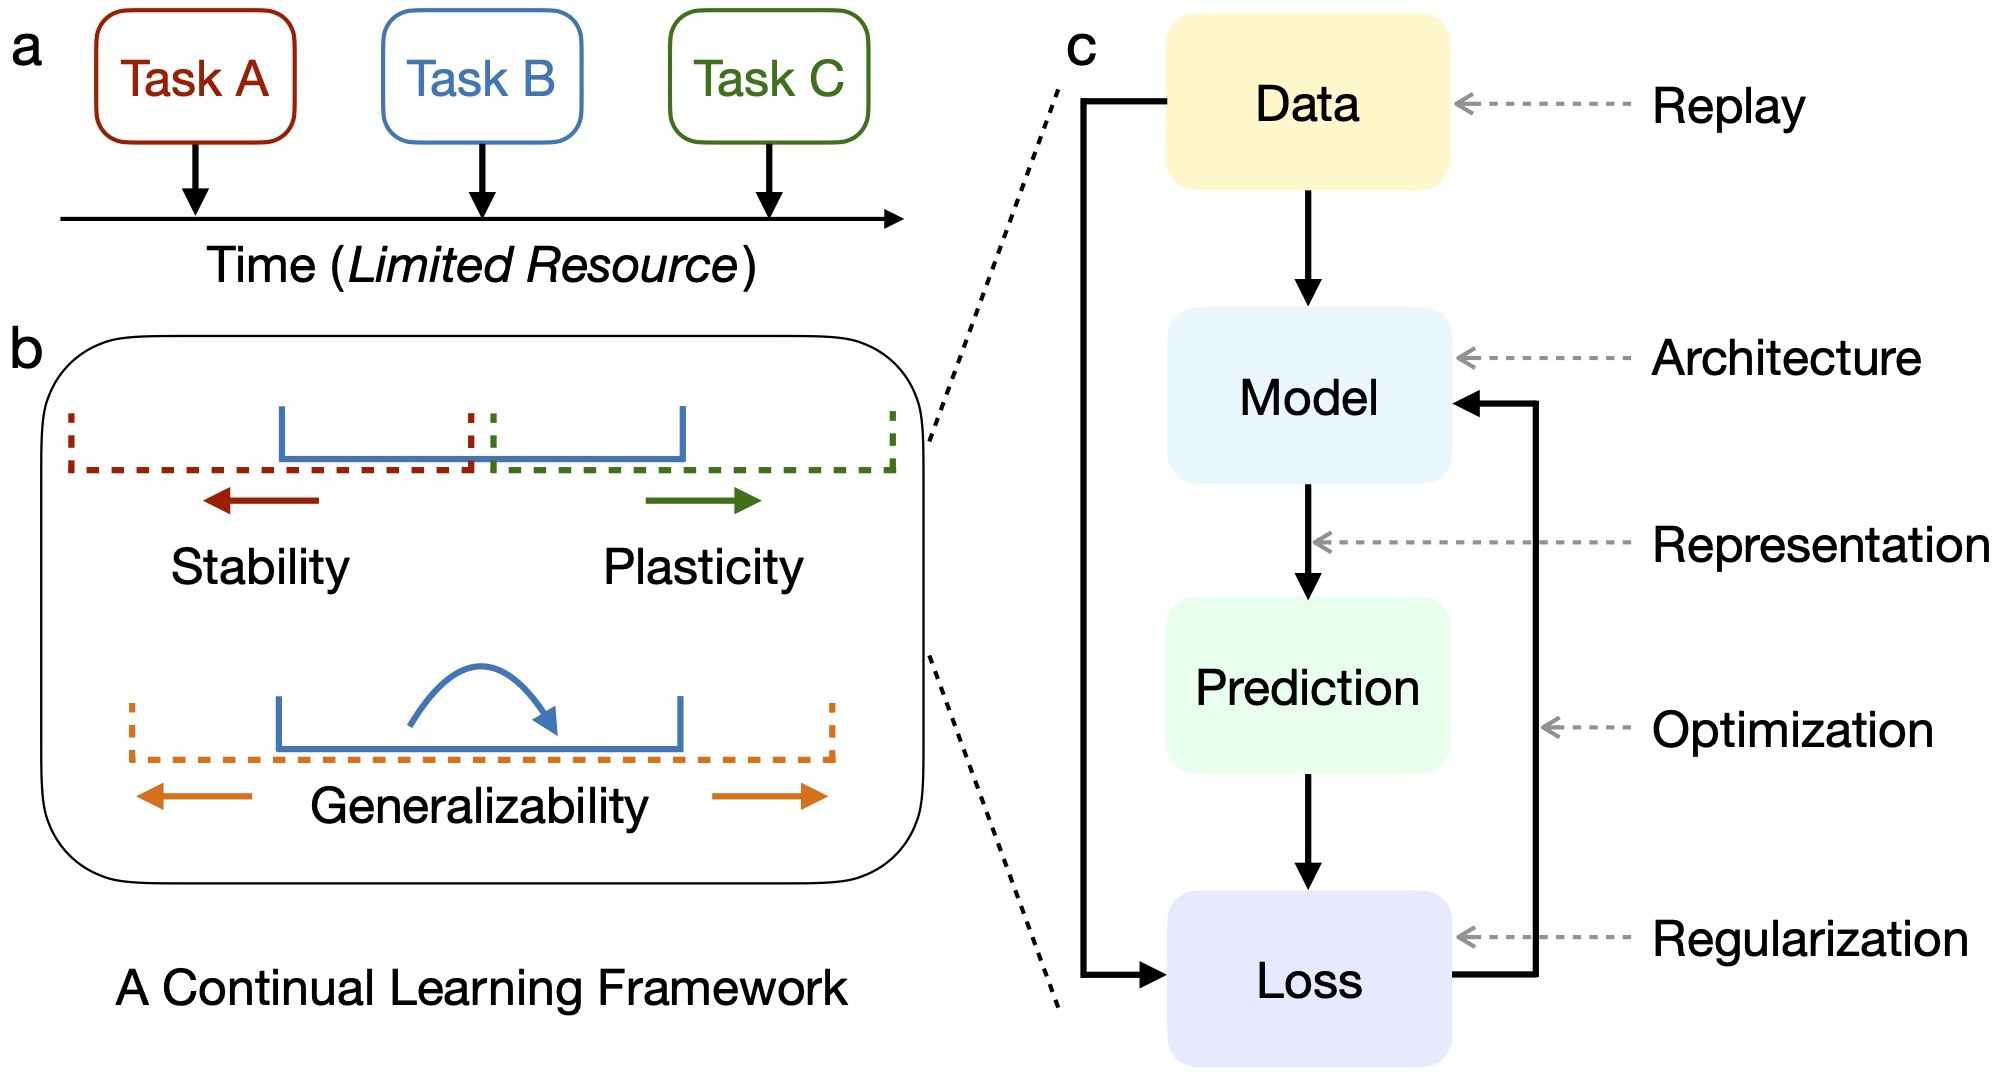
\includegraphics[width=0.7\linewidth]{imgs/continual_learning/cl_1.png}
    \caption{A conceptual framework of continual learning. \textbf{a}, Continual learning requires adapting to incremental tasks with dynamic data distributions. \textbf{b}, A desirable solution should ensure a proper balance between stability (red arrow) and plasticity (green arrow), as well as an adequate generalizability to intra-task (blue arrow) and inter-task (orange arrow) distribution differences. \textbf{c}, Representative strategies have targeted various aspects of machine learning.}
    \label{fig:cl_1}
\end{figure}

Numerous efforts have been devoted to addressing the above challenges, which can be conceptually separated into five groups (Fig.\ref{fig:cl_1}, c): \textit{regularization-based approach}; \textit{replay-based approach}; \textit{optimization-based approach}; \textit{representation-based approach}; and \textit{architecture-based approach}. These methods are \textit{closely connected}, e.g., regularization and replay ultimately act to rectify the gradient directions, and \textit{highly synergistic}, e.g., the efficacy of replay can be facilitated by distilling knowledge from the old model.

\section{Setup}
In this section, we first present a basic formulation of continual leanring. Then we introduce typical scenairos and evaluation metrics.

\subsection{Basic Formulation}
A continual learning model parameterized by \(\theta\) needs to learn corresponding task(s) with no or limited access to old training samples and perform well on their test sets. Formally, an incoming batch of training samples belonging to a task \(t\) can be represented as \(\mathcal{D}_{t, b}=\left\{\mathcal{X}_{t, b}, \mathcal{Y}_{t, b}\right\}\) where \(\mathcal{X}_{t, b}\) is the input data, \(\mathcal{Y}_{t, b}\) is the data label, \(t \in \mathcal{T}=\{1, \cdots, k\}\) is the task identity and \(b \in \mathcal{B}_{t}\) is the batch index ( \(\mathcal{T}\) and \(\mathcal{B}_{t}\) denote their space, respectively). Here we define a "task" by its training samples \(\mathcal{D}_{t}\) following the distribution \(\mathbb{D}_{t}:=p\left(\mathcal{X}_{t}, \mathcal{Y}_{t}\right)\left(\mathcal{D}_{t}\right.\) denotes the entire training set by omitting the batch index, likewise for \(\mathcal{X}_{t}\) and \(\left( \mathcal{Y}_{t}\right)\), and assume that there is no difference in distribution between training and testing. Under realistic constraints, the data label \(\mathcal{Y}_{t}\) and the task identity \(t\) might not be always available. In continual learning, the training samples of each task can arrive incrementally in batches (i.e., \(\left\{\left\{\mathcal{D}_{t, b}\right\}_{b \in \mathcal{B}_{t}}\right\}_{t \in \mathcal{T}}\) ) or simultaneously (i.e.,\(\left\{\mathcal{D}_{t}\right\}_{t \in \mathcal{T}}\)).

\begin{table}[H]
    \centering
    \renewcommand{\arraystretch}{1.75}
    \resizebox{\textwidth}{!}{
        \begin{tabular}{c|c|c}
            \hline
            \textbf{Scenario} & \textbf{Training}                                                                                                                                                                                                                               & \textbf{Testing}                                                                                  \\
            \hline IIL        & \(\left\{\left\{\mathcal{D}_{t, b}, t\right\}_{b \in \mathcal{B}_{t}}\right\}_{t=j}\)                                                                                                                                                           & \(\left\{p\left(\mathcal{X}_{t}\right)\right\}_{t=j ; t}\) is not required                        \\
            \hline DIL        & \(\left\{\mathcal{D}_{t}, t\right\}_{t \in \mathcal{T}} ; p\left(\mathcal{X}_{i}\right) \neq p\left(\mathcal{X}_{j}\right)\) and \(\mathcal{Y}_{i}=\mathcal{Y}_{j}\) for \(i \neq j\)                                                           & \(\left\{p\left(\mathcal{X}_{t}\right)\right\}_{t \in \mathcal{T}}, t\) is not required           \\
            \hline TIL        & \(\left\{\mathcal{D}_{t}, t\right\}_{t \in \mathcal{T}} ; p\left(\mathcal{X}_{i}\right) \neq p\left(\mathcal{X}_{j}\right)\) and \(\mathcal{Y}_{i} \cap \mathcal{Y}_{j}=\emptyset\) for \(i \neq j\)                                            & \(\left\{p\left(\mathcal{X}_{t}\right)\right\}_{t \in \mathcal{T} ; t}\) is available             \\
            \hline CIL        & \(\left\{\mathcal{D}_{t}, t\right\}_{t \in \mathcal{T}} ; p\left(\mathcal{X}_{i}\right) \neq p\left(\mathcal{X}_{j}\right)\) and \(\mathcal{Y}_{i} \cap \mathcal{Y}_{j}=\emptyset\) for \(i \neq j\)                                            & \(\left\{p\left(\mathcal{X}_{t}\right)\right\}_{t \in \mathcal{T} ; t}\) is unavailable           \\
            \hline TFCL       & \(\left\{\left\{\mathcal{D}_{t, b}\right\}_{b \in \mathcal{B}_{t}}\right\}_{t \in \mathcal{T}} ; p\left(\mathcal{X}_{i}\right) \neq p\left(\mathcal{X}_{j}\right)\) and \(\mathcal{Y}_{i} \cap \mathcal{Y}_{j}=\emptyset\) for \(i \neq j\)     & \(\left\{p\left(\mathcal{X}_{t}\right)\right\}_{t \in \mathcal{T}} ; t\) is optionally available  \\ \hline OCL  & \(\left\{\left\{\mathcal{D}_{t, b}\right\}_{b \in \mathcal{B}_{t}}\right\}_{t \in \mathcal{T}},|b|=1 ; p\left(\mathcal{X}_{i}\right) \neq p\left(\mathcal{X}_{j}\right)\) and \(\mathcal{Y}_{i} \cap \mathcal{Y}_{j}=\emptyset\) for \(i \neq j\) & \(\left\{p\left(\mathcal{X}_{t}\right)\right\}_{t \in \mathcal{T}} ; t\) is optionally available \\
            \hline BBCL       & \(\left\{\mathcal{D}_{t}, t\right\}_{t \in \mathcal{T}} ; p\left(\mathcal{X}_{i}\right) \neq p\left(\mathcal{X}_{j}\right), \mathcal{Y}_{i} \neq \mathcal{Y}_{j}\) and \(\mathcal{Y}_{i} \cap \mathcal{Y}_{j} \neq \emptyset\) for \(i \neq j\) & \(\left\{p\left(\mathcal{X}_{t}\right)\right\}_{t \in \mathcal{T} ; t \text { is unavailable }}\) \\
            \hline CPT        & \(\left\{\mathcal{D}_{t}^{p t}, t\right\}_{t \in \mathcal{T} p t}\), followed by a downstream task \(j\)                                                                                                                                        & \(\left\{p\left(\mathcal{X}_{t}\right)\right\}_{t=j ; t}\) is not required                        \\
            \hline\end{tabular}}
    \caption{A formal comparison of typical continual learning scenarios. \(\mathcal{D}_{t, b}:\) the training samples of task \(t\) and batch \(b\). \(|b|:\) the size of batch \(b\). \(\mathcal{B}_{t}:\) the space of incremental batches belonging to task \(t\). \(\mathcal{D}_{t}:\) the training set of task \(t\) (further specified as \(\mathcal{D}_{t}^{p t}\) for pre-training). \(\mathcal{T}:\) the space of all incremental tasks (further specified as \(\mathcal{T}^{p t}\) for pre-training). \(\mathcal{X}_{t}:\) the input data in \(\mathcal{D}_{t}\), \(p\left(\mathcal{X}_{t}\right):\) the distribution of \(\mathcal{X}_{t} . \mathcal{Y}_{t}:\) the data label of \(\mathcal{X}_{t}\).}
    \label{table:4.1}
\end{table}

\subsection{Typical Scenairo}

Detail of some tyical continual learning scenairos (refer to Table \ref{table:4.1} for a formal comparision):
\begin{itemize}
    \item \textit{Instance-Incremental Learning} (IIL): All training samples belong to the same task and arrive in batches.
    \item \textit{Domain-Incremental Learning} (DIL): Tasks have the same data label space but different input distributions. Task identities are not required.
    \item \textit{Task-Incremental Learning} (TIL): Tasks have disjoint data label spaces. Task identities are provided in both training and testing.
    \item \textit{Class-Incremental Learning} (CIL): Tasks have disjoint data label spaces. Task identities are only provided in training.
\end{itemize}
